\documentclass[a4paper, 11pt]{article}
\usepackage[spanish]{babel}
\selectlanguage{spanish}
\usepackage{graphicx}
\usepackage{wrapfig}
\usepackage[utf8]{inputenc}
\usepackage{amsmath}
\usepackage{dsfont}
\usepackage{multirow}
\usepackage{vmargin}
\usepackage{subfigure}
\usepackage[numbers, sort&compress]{natbib}
\usepackage{url}
\usepackage{cite}
\usepackage{wrapfig}
\usepackage{enumerate} 
\usepackage{sectsty} % centrar secciones de encabezados
\usepackage[usenames]{color}
\usepackage{caption}
\usepackage{amsfonts}
\usepackage{amssymb}
\usepackage{listings}
\usepackage{color}
\usepackage{algpseudocode}
\usepackage{multirow}
\usepackage[usenames]{color}
\usepackage{epstopdf}
\usepackage{float}
\usepackage{nameref}
\spanishdecimal{.}

\setmargins
{2.5cm}                        % margen izquierdo
{1cm}                         % margen superior
{16.5cm}                      % anchura del texto
{23.42cm}                    % altura del texto
{10pt}                           % altura de los encabezados
{0cm}                           % espacio entre el texto y los encabezados
{0pt}                             % altura del pie de página
{1cm}                           % espacio entre el texto y el pie de página

\definecolor{mygreen}{rgb}{0,0.6,0}
\definecolor{mygray}{rgb}{0.5,0.5,0.5}
\definecolor{mymauve}{rgb}{0.58,0,0.82}

\lstset{ 
  backgroundcolor=\color{white},   % choose the background color; you must add \usepackage{color} or \usepackage{xcolor}; should come as last argument
  basicstyle=\footnotesize,        % the size of the fonts that are used for the code
  breakatwhitespace=false,         % sets if automatic breaks should only happen at whitespace
  breaklines=true,                 % sets automatic line breaking
  captionpos=b,                    % sets the caption-position to bottom
  commentstyle=\color{mygreen},    % comment style
  deletekeywords={...},            % if you want to delete keywords from the given language
  escapeinside={\%*}{*)},          % if you want to add LaTeX within your code
  extendedchars=true,              % lets you use non-ASCII characters; for 8-bits encodings only, does not work with UTF-8
  firstnumber=1,                % start line enumeration with line 1000
  frame=single,	                   % adds a frame around the code
  keepspaces=true,                 % keeps spaces in text, useful for keeping indentation of code (possibly needs columns=flexible)
  keywordstyle=\color{blue},       % keyword style
  language=Octave,                 % the language of the code
  morekeywords={*,...},            % if you want to add more keywords to the set
  numbers=left,                    % where to put the line-numbers; possible values are (none, left, right)
  numbersep=5pt,                   % how far the line-numbers are from the code
  numberstyle=\tiny\color{mygray}, % the style that is used for the line-numbers
  rulecolor=\color{black},         % if not set, the frame-color may be changed on line-breaks within not-black text (e.g. comments (green here))
  showspaces=false,                % show spaces everywhere adding particular underscores; it overrides 'showstringspaces'
  showstringspaces=false,          % underline spaces within strings only
  showtabs=false,                  % show tabs within strings adding particular underscores
  stepnumber=1,                    % the step between two line-numbers. If it's 1, each line will be numbered
  stringstyle=\color{mymauve},     % string literal style
  tabsize=2,	                   % sets default tabsize to 2 spaces
  title=\lstname                   % show the filename of files included with \lstinputlisting; also try caption instead of title
}


\begin{document}

\title{Medición de tiempo de ejecución}
\author{Matr\'icula: 1985281}
\date{ }
\maketitle

\vspace{-1 cm}
\begin{center}\rule{\textwidth}{0.1mm} \end{center}
\vspace{-1.3 cm}
\begin {center}
\item \Large{\textbf{ Resumen}}
\end {center}

Este trabajo busca resolver grafos con la implementación de los algoritmos  de \color{blue}NetworkX\color{black}  \  de \color{blue} \texttt{Python}\color{black}. Se seleccionan algunos grafos de la tarea 2 y se generan otros, para así poder resolver cinco grafos distintos para cada uno de los cinco algoritmos seleccionados.
\vspace{-0.5cm}
\begin{center}\rule{\textwidth}{0.1mm} \end{center}




\section*{\centering{Introducción}}
La librería \color{blue}NetworkX\color{black} \ de \color{blue}\texttt{Python} \color{black} \ proporciona algoritmos para resolver diversos problemas, de los cuales se escogieron los siguientes cinco:

\begin{itemize}
\item Centralidad intermedia: Calcula la centralidad de intermediación de rutas más cortas para todos los nodos.
\item Árbol de expansión mínimo: Calcula un árbol  de expansión mínimo del grafo.
\item Flujo máximo: Calcula el flujo máximo de un nodo a otro.
\item Ruta mas corta: Calcula las rutas más cortas entre los nodos del grafo.
\item Coloración glotona: Colorea una gráfica usando varias estrategias de coloración codiciosa.
\end{itemize}


\section*{\centering{Metodología y Resultados}}

Se seleccionan algunos grafos utilizados en la tarea 2 y se generan otros grafos que son compatibles con los requerimientos que el algoritmo tiene sobre sus datos de entrada, se repite cada ejecución por la cantidad suficiente de veces para que el tiempo total de ejecución del conjunto de réplicas sea mayor a cinco segundos (se sube el número de réplicas hasta que esto se logre). Luego se repite la medición del conjunto de réplicas hasta treinta veces en total, sin exceder quince minutos de tiempo total de ejecución.
\\
\\
Después con la ayuda de librerías adicionales tales como \color{blue}\texttt{NumPy}\color{black} \ y \color{blue}\texttt{SciPy}\color{black}, se calcula para cada algoritmo el promedio $(\mu)$ y desviación estándar $(\sigma)$  de la ejecución del conjunto de réplicas y se grafica un histograma de las mediciones individuales para cada algoritmo.

\begin{lstlisting}[language=Python]
import networkx as nx
import matplotlib.pyplot as plt
import time
import numpy as np
from scipy import stats
\end{lstlisting}

\subsection*{\centering{Centralidad intermedia}}

La figura [\ref{figure1}.b] muestra la centralidad intermedia para cada nodo del grafo ejemplo de redes sociales de la tarea 2.

\begin{lstlisting}[language=Python]
b_w = nx.betweenness_centrality(G1)
\end{lstlisting}

\begin{figure}[H]
\centering
\subfigure[Versión primaria]{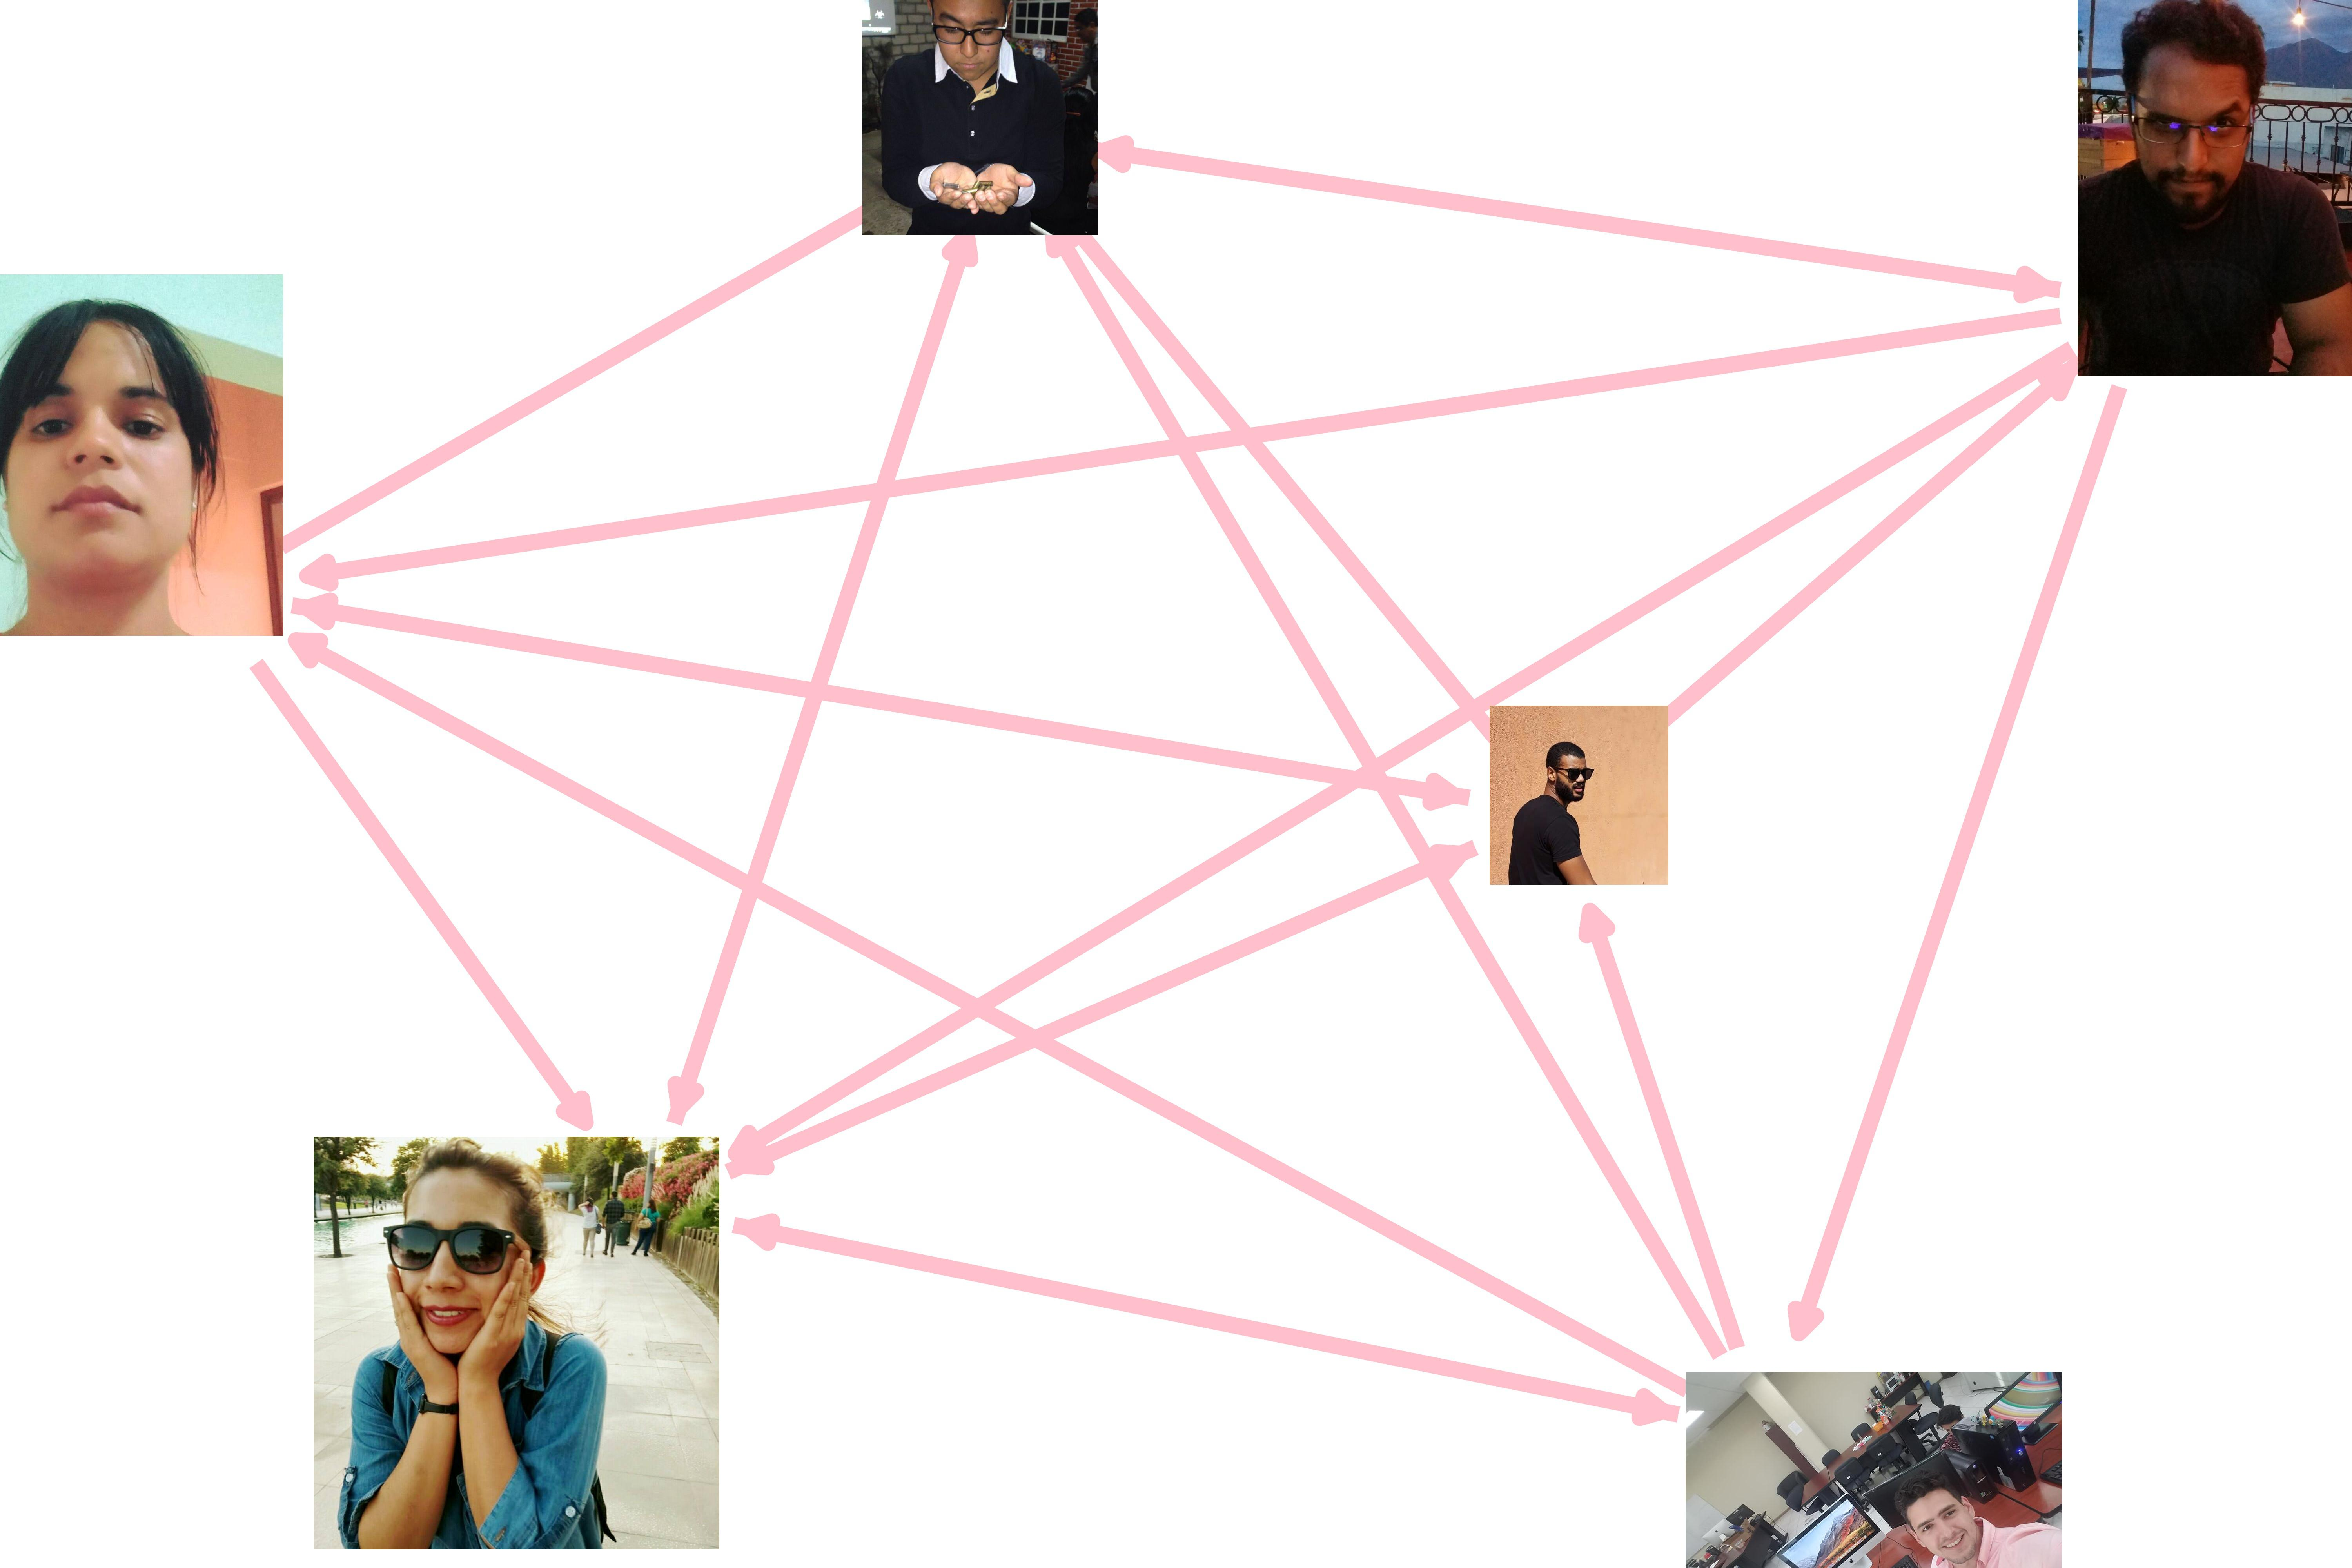
\includegraphics[width=60mm]{./original1}}
\subfigure[\texttt{betweenness\_centrality}]{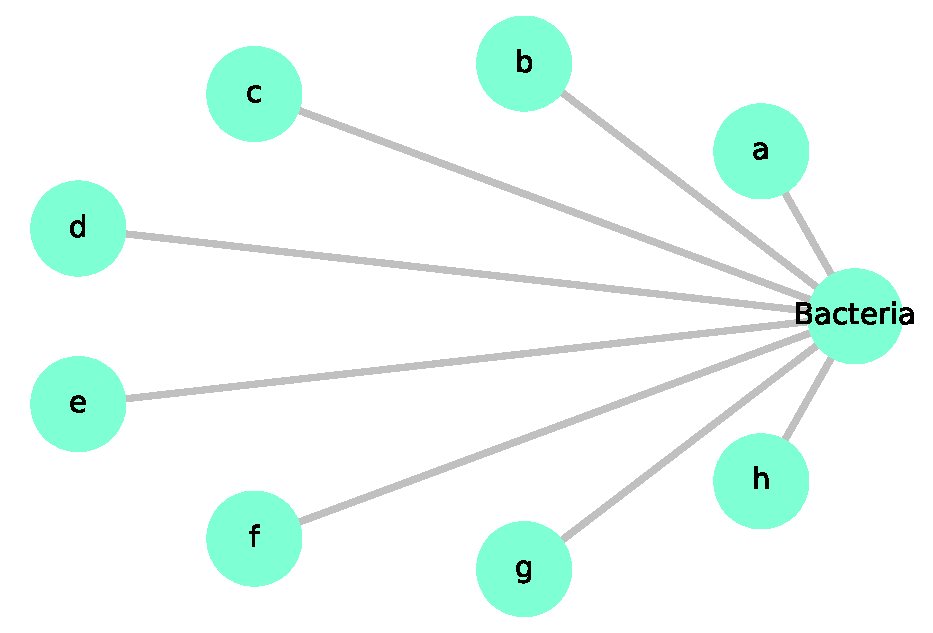
\includegraphics[width=80mm]{./grafo11}}
\caption{Ejemplo de redes sociales} \label{figure1}
\end{figure}

También, otro grafo utilizado para aplicar este algoritmo es el famoso grafo de la red social \textit{Krackhardt Kite}, una red social de diez actores presentada por David Krackhardt para ilustrar centralidad intermedia. Véase figura [\ref{figure2}].

\begin{figure}[H]
\centering
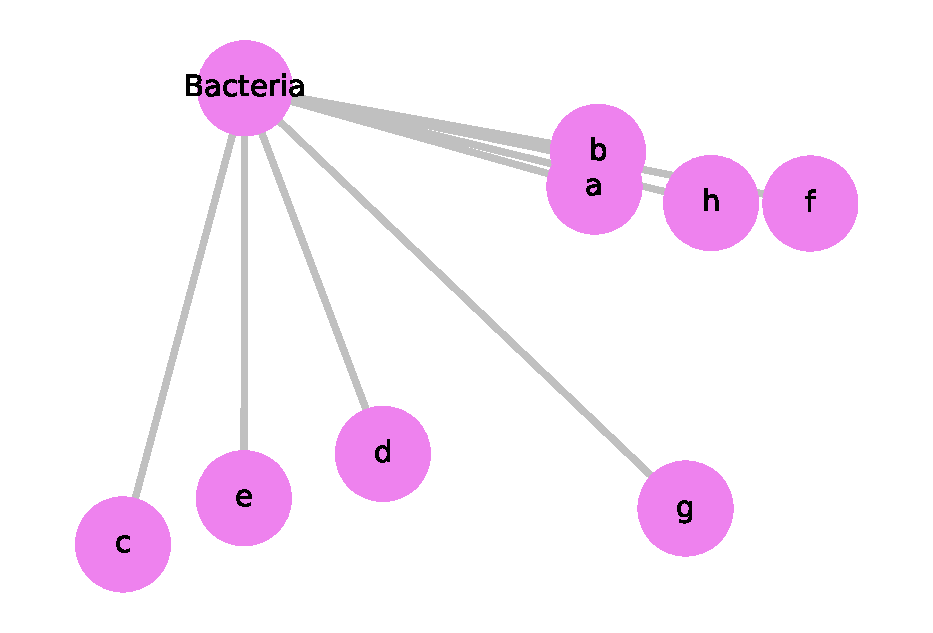
\includegraphics[width=100mm]{grafo12}
\caption{Red social de Krackhardt Kite} \label{figure2}
\end{figure}

Ahora se calcula para el algoritmo, el promedio y desviación estándar de la ejecución del conjunto de réplicas y se grafica un histograma.

\begin{figure}[H]
\centering
\subfigure[Histograma]{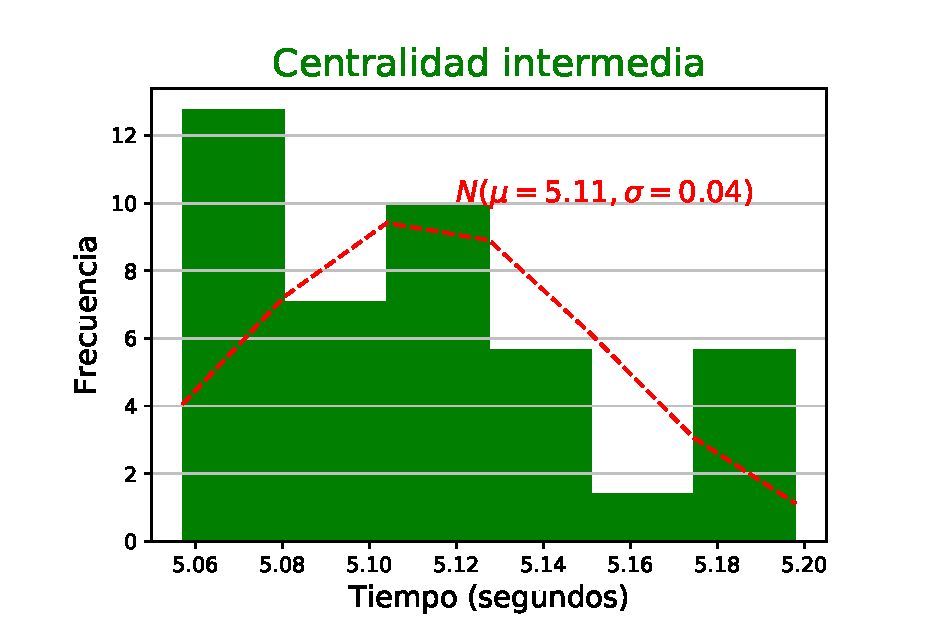
\includegraphics[width=70mm]{./histograma1}}
\subfigure[Diagrama de caja y bigotes]{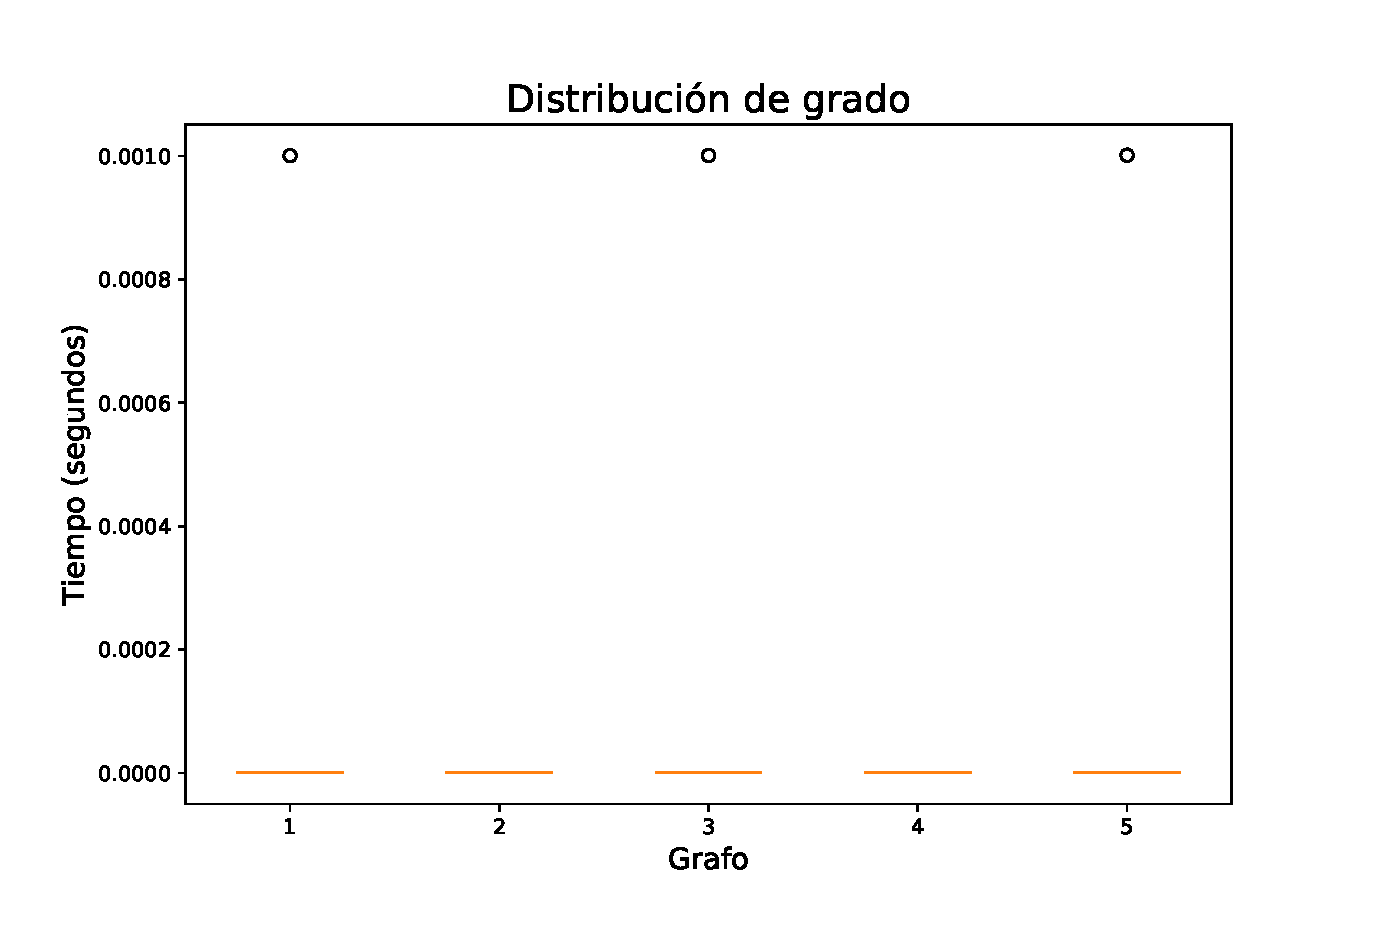
\includegraphics[width=90mm]{./boxplot1}}
\caption{Histograma y diagrama de caja y bigotes} \label{figure3}
\end{figure}

En la figura [\ref{figure3}.a] se muestra el histograma de los tiempos promedio del algoritmo y se calcula el promedio $(\mu)$ y la desviación estándar $(\sigma)$ para graficar la línea punteada que corresponde a la distribución normal $N\sim(\mu=\frac{\sum_{i=1}^n x_{i}}{n}=5.11, \sigma=\frac{\sum_{i=1}^n {(x_{i}-\mu)}^2}{n}=0.04)$ y se puede ver que la línea punteada no se ajusta al histograma por lo que se realiza la prueba estadística \textit{Shapiro-Wilk} para checar la normalidad de los datos.

\begin{lstlisting}[language=Python]
stats.shapiro(tiempos_algoritmo_1)
\end{lstlisting}

\noindent\fbox{
\begin{minipage}{\textwidth}
\begin{algorithmic}
\State{\texttt{\color{blue}In:\color{black} \ stats.shapiro} (tiempos\_algoritmo\_1) \ \ \ \ \ \ \ \texttt{\color{blue}Out:\color{black} \ $(W=0.6412,p= 2.4210 \cdot {10}^{-7})$}}
\end{algorithmic}
\end{minipage}
}
\\
\\
La prueba muestra que el p-valor es menor a 0.05 (nivel de significancia), entonces la hipótesis nula es rechazada (se concluye que los datos no vienen de una distribución normal).
\\
\\
Por otro lado en la figura [\ref{figure3}.b] se muestran los diagramas de caja y bigotes para los tiempos individuales de los cinco grafos utilizados en el algoritmo, el número rojo representa la cantidad de nodos del grafo y se puede apreciar que conforme aumenta la cantidad de nodos en el grafo, los tiempos computacionales también crecen.


\newpage


\subsection*{\centering{Árbol de expansión mínimo}}

La figura [\ref{figure4}] muestra ejemplos de grafos y sus respectivos grafos  de árboles de expansión mínima.

\begin{lstlisting}[language=Python]
T1 = nx.minimum_spanning_tree(G6)
\end{lstlisting}

\begin{figure}[H]
\centering
\subfigure[Puentes de \textit{Könisberg}]{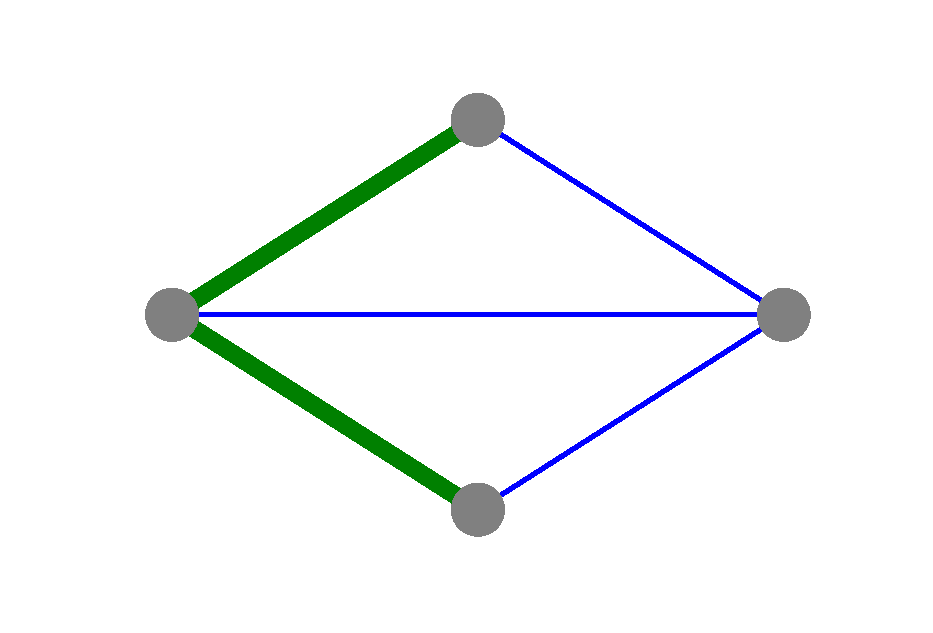
\includegraphics[width=60mm]{./original2}}
\subfigure[Árbol de expansión mínima de (a)]{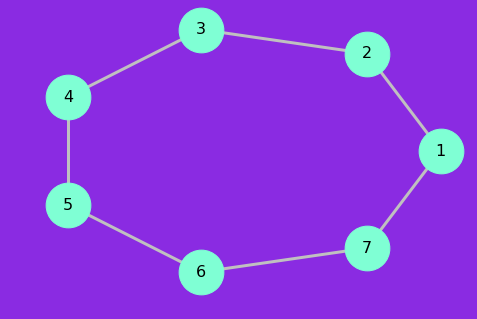
\includegraphics[width=60mm]{./grafo21}}
\subfigure[Grafo de 100 nodos]{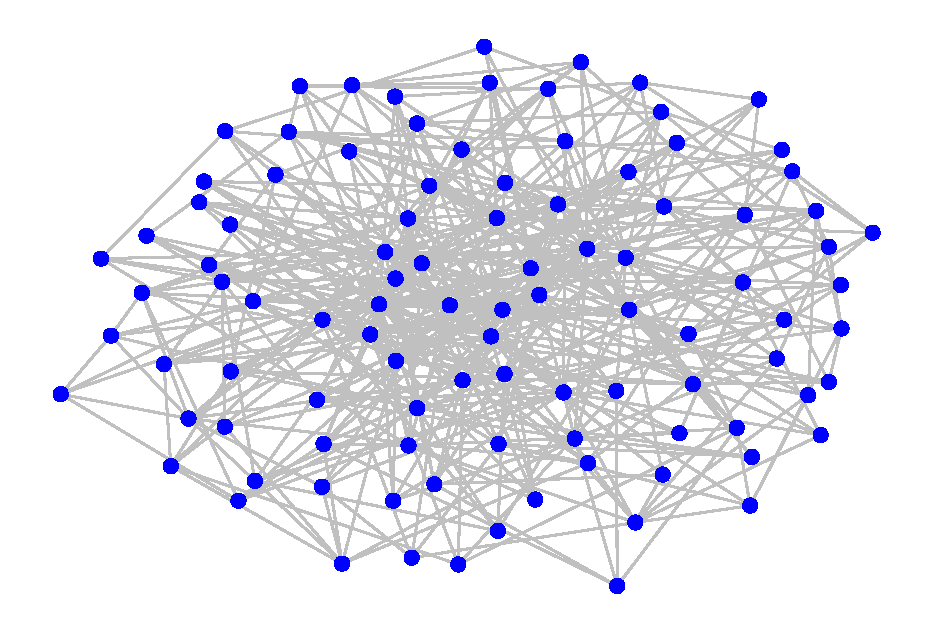
\includegraphics[width=60mm]{./grafo24}}
\subfigure[Árbol de expansión mínima de (c)]{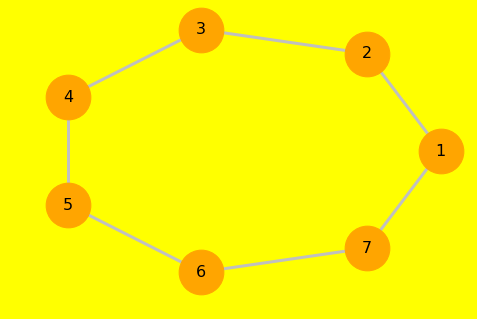
\includegraphics[width=60mm]{./grafo25}}
\caption{Ejemplos de árbol de expansión mínima} \label{figure4}
\end{figure}

Ahora se calcula para el algoritmo, el promedio y desviación estándar de la ejecución del conjunto de réplicas y se grafica un histograma.

\begin{figure}[H]
\centering
\subfigure[Histograma]{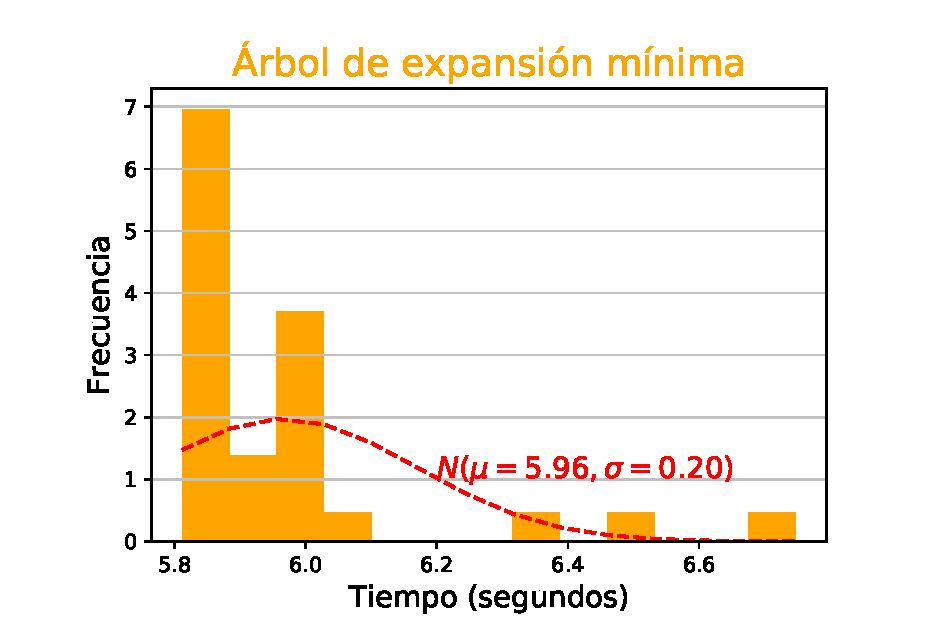
\includegraphics[width=70mm]{./histograma2}}
\subfigure[Diagrama de caja y bigotes]{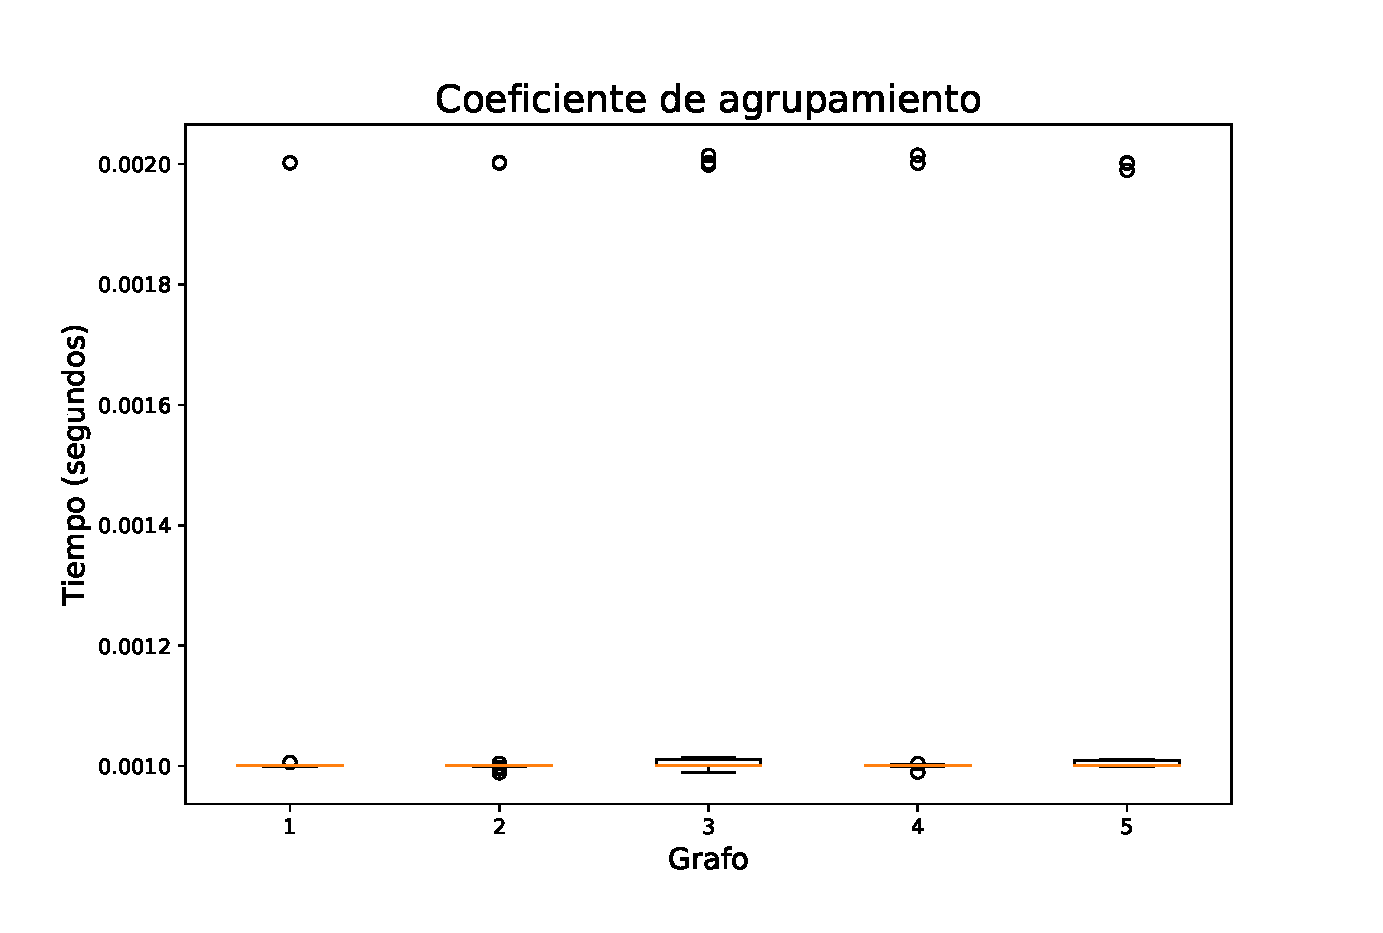
\includegraphics[width=90mm]{./boxplot2}}
\caption{Histograma y diagrama de caja y bigotes} \label{figure5}
\end{figure}

En la figura [\ref{figure5}.a] se muestra el histograma de los tiempos promedio del algoritmo y se calcula el promedio $(\mu)$ y la desviación estándar $(\sigma)$ para graficar la línea punteada que corresponde a la distribución normal $N\sim(\mu=5.96, \sigma=0.20)$ y se puede ver que la línea punteada no se ajusta al histograma por lo que se realiza la prueba estadística \textit{Shapiro-Wilk} para checar la normalidad de los datos.
\\
\\
\noindent\fbox{
\begin{minipage}{\textwidth}
\begin{algorithmic}
\State{\texttt{\color{blue}In:\color{black} \ stats.shapiro} (tiempos\_algoritmo\_2) \ \ \ \ \ \ \ \texttt{\color{blue}Out:\color{black} \ $(W=0.5320,p=  1.1895 \cdot {10}^{-8})$}}
\end{algorithmic}
\end{minipage}
}
\\
\\
La prueba muestra que el p-valor es menor a 0.05 (nivel de significancia), entonces la hipótesis nula es rechazada (se concluye que los datos no vienen de una distribución normal).
\\
\\
Por otro lado en la figura [\ref{figure5}.b] se muestran los diagramas de caja y bigotes para los tiempos individuales de los cinco grafos utilizados en el algoritmo, el número rojo representa la cantidad de nodos del grafo y se puede apreciar que conforme aumenta la cantidad de nodos en el grafo, los tiempos computacionales también crecen.






\subsection*{\centering{Flujo máximo}}

En este ejemplo se le pide al algoritmo de flujo máximo encontrar el flujo máximo del nodo uno al nodo diez del grafo llamado G11.
\begin{lstlisting}[language=Python]
 MF_1 = nx.maximum_flow(G11, 1, 10, capacity='capacidad', flow_func=None)
\end{lstlisting}

Ahora se calcula para el algoritmo, el promedio y desviación estándar de la ejecución del conjunto de réplicas y se grafica un histograma.

\begin{figure}[H]
\centering
\subfigure[Histograma]{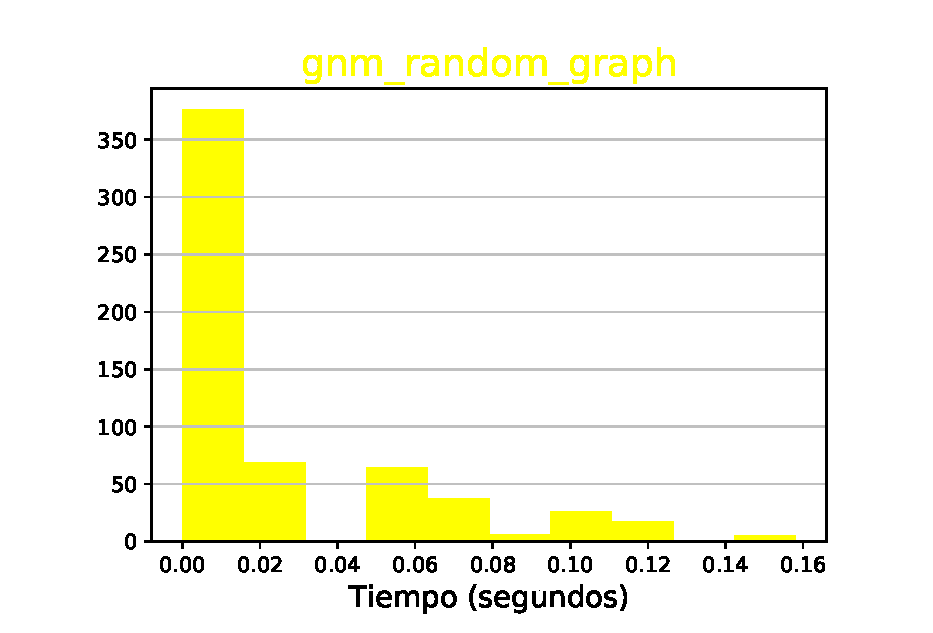
\includegraphics[width=70mm]{./histograma3}}
\subfigure[Diagrama de caja y bigotes]{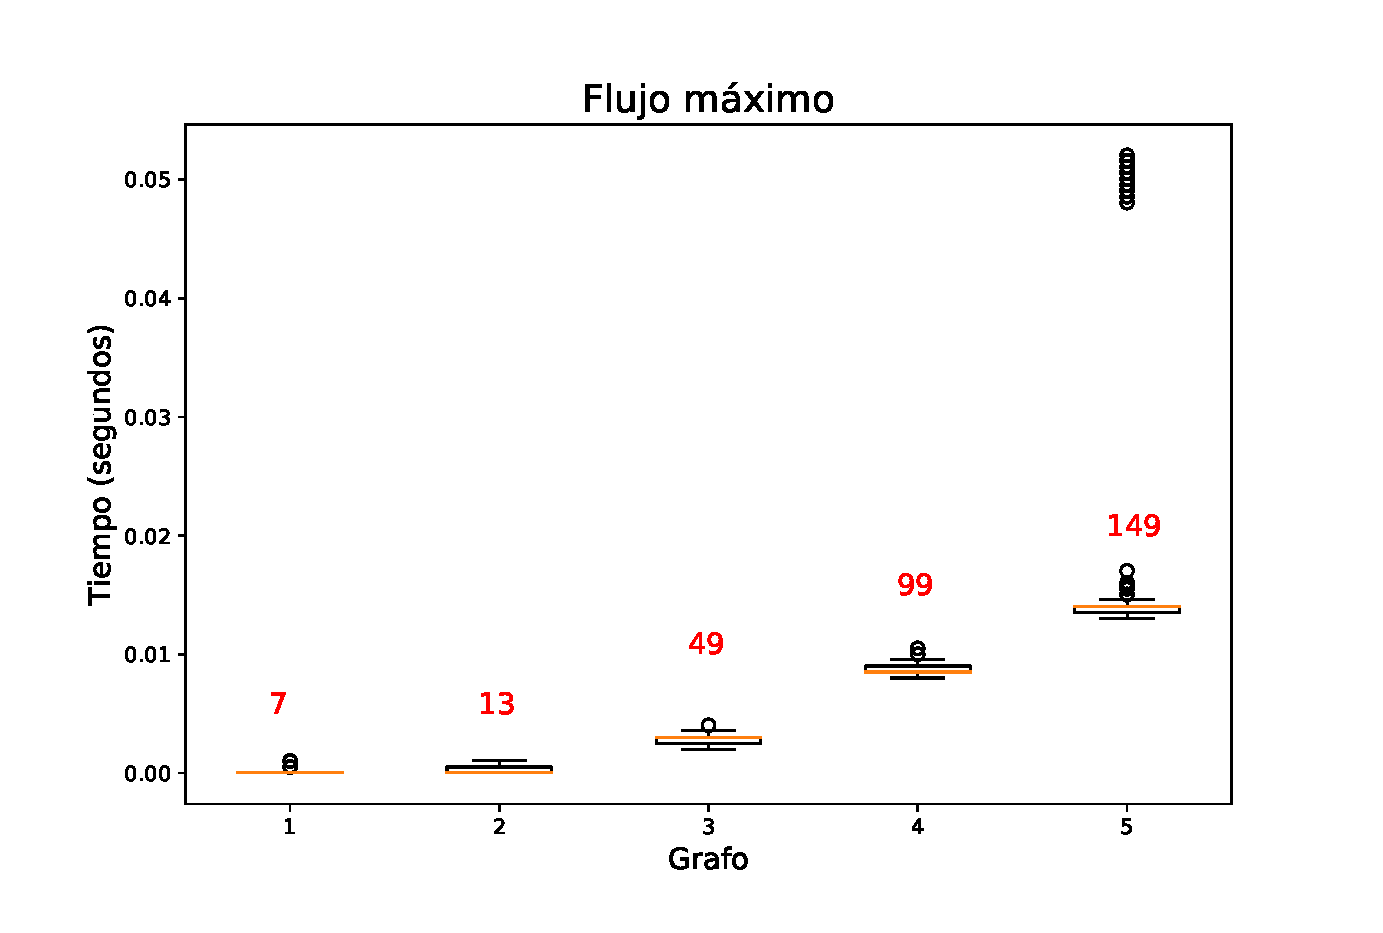
\includegraphics[width=90mm]{./boxplot3}}
\caption{Histograma y diagrama de caja y bigotes} \label{figure6}
\end{figure}

En la figura [\ref{figure6}.a] se muestra el histograma de los tiempos promedio del algoritmo y se calcula el promedio $(\mu)$ y la desviación estándar $(\sigma)$ para graficar la línea punteada que corresponde a la distribución normal $N\sim(\mu=5.25, \sigma=0.55)$ y se puede ver que la línea punteada no se ajusta al histograma por lo que se realiza la prueba estadística \textit{Shapiro-Wilk} para checar la normalidad de los datos.
\\
\\
\noindent\fbox{
\begin{minipage}{\textwidth}
\begin{algorithmic}
\State{\texttt{\color{blue}In:\color{black} \ stats.shapiro} (tiempos\_algoritmo\_3) \ \ \ \ \ \ \ \texttt{\color{blue}Out:\color{black} \ $(W=0.8749,p=  0.0021)$}}
\end{algorithmic}
\end{minipage}
}
\\
\\
La prueba muestra que el p-valor es menor a 0.05 (nivel de significancia), entonces la hipótesis nula es rechazada (se concluye que los datos no vienen de una distribución normal).
\\
\\
Por otro lado en la figura [\ref{figure6}.b] se muestran los diagramas de caja y bigotes para los tiempos individuales de los cinco grafos utilizados en el algoritmo, el número rojo representa la cantidad de nodos del grafo y se puede apreciar que conforme aumenta la cantidad de nodos en el grafo, los tiempos computacionales también crecen.







\subsection*{\centering{Ruta mas corta}}

La figura [\ref{figure7}] muestra un ejemplo de un grafo y sus respectivas rutas mas cortas del nodo uno al nodo siete del grafo llamado G16.

\begin{lstlisting}[language=Python]
rutas1 = [p for p in nx.all_shortest_paths(G16, source=1, target=7, weight=None,method='dijkstra')]

\end{lstlisting}

\begin{figure}[H]
\centering
\subfigure[Grafo de 30 nodos]{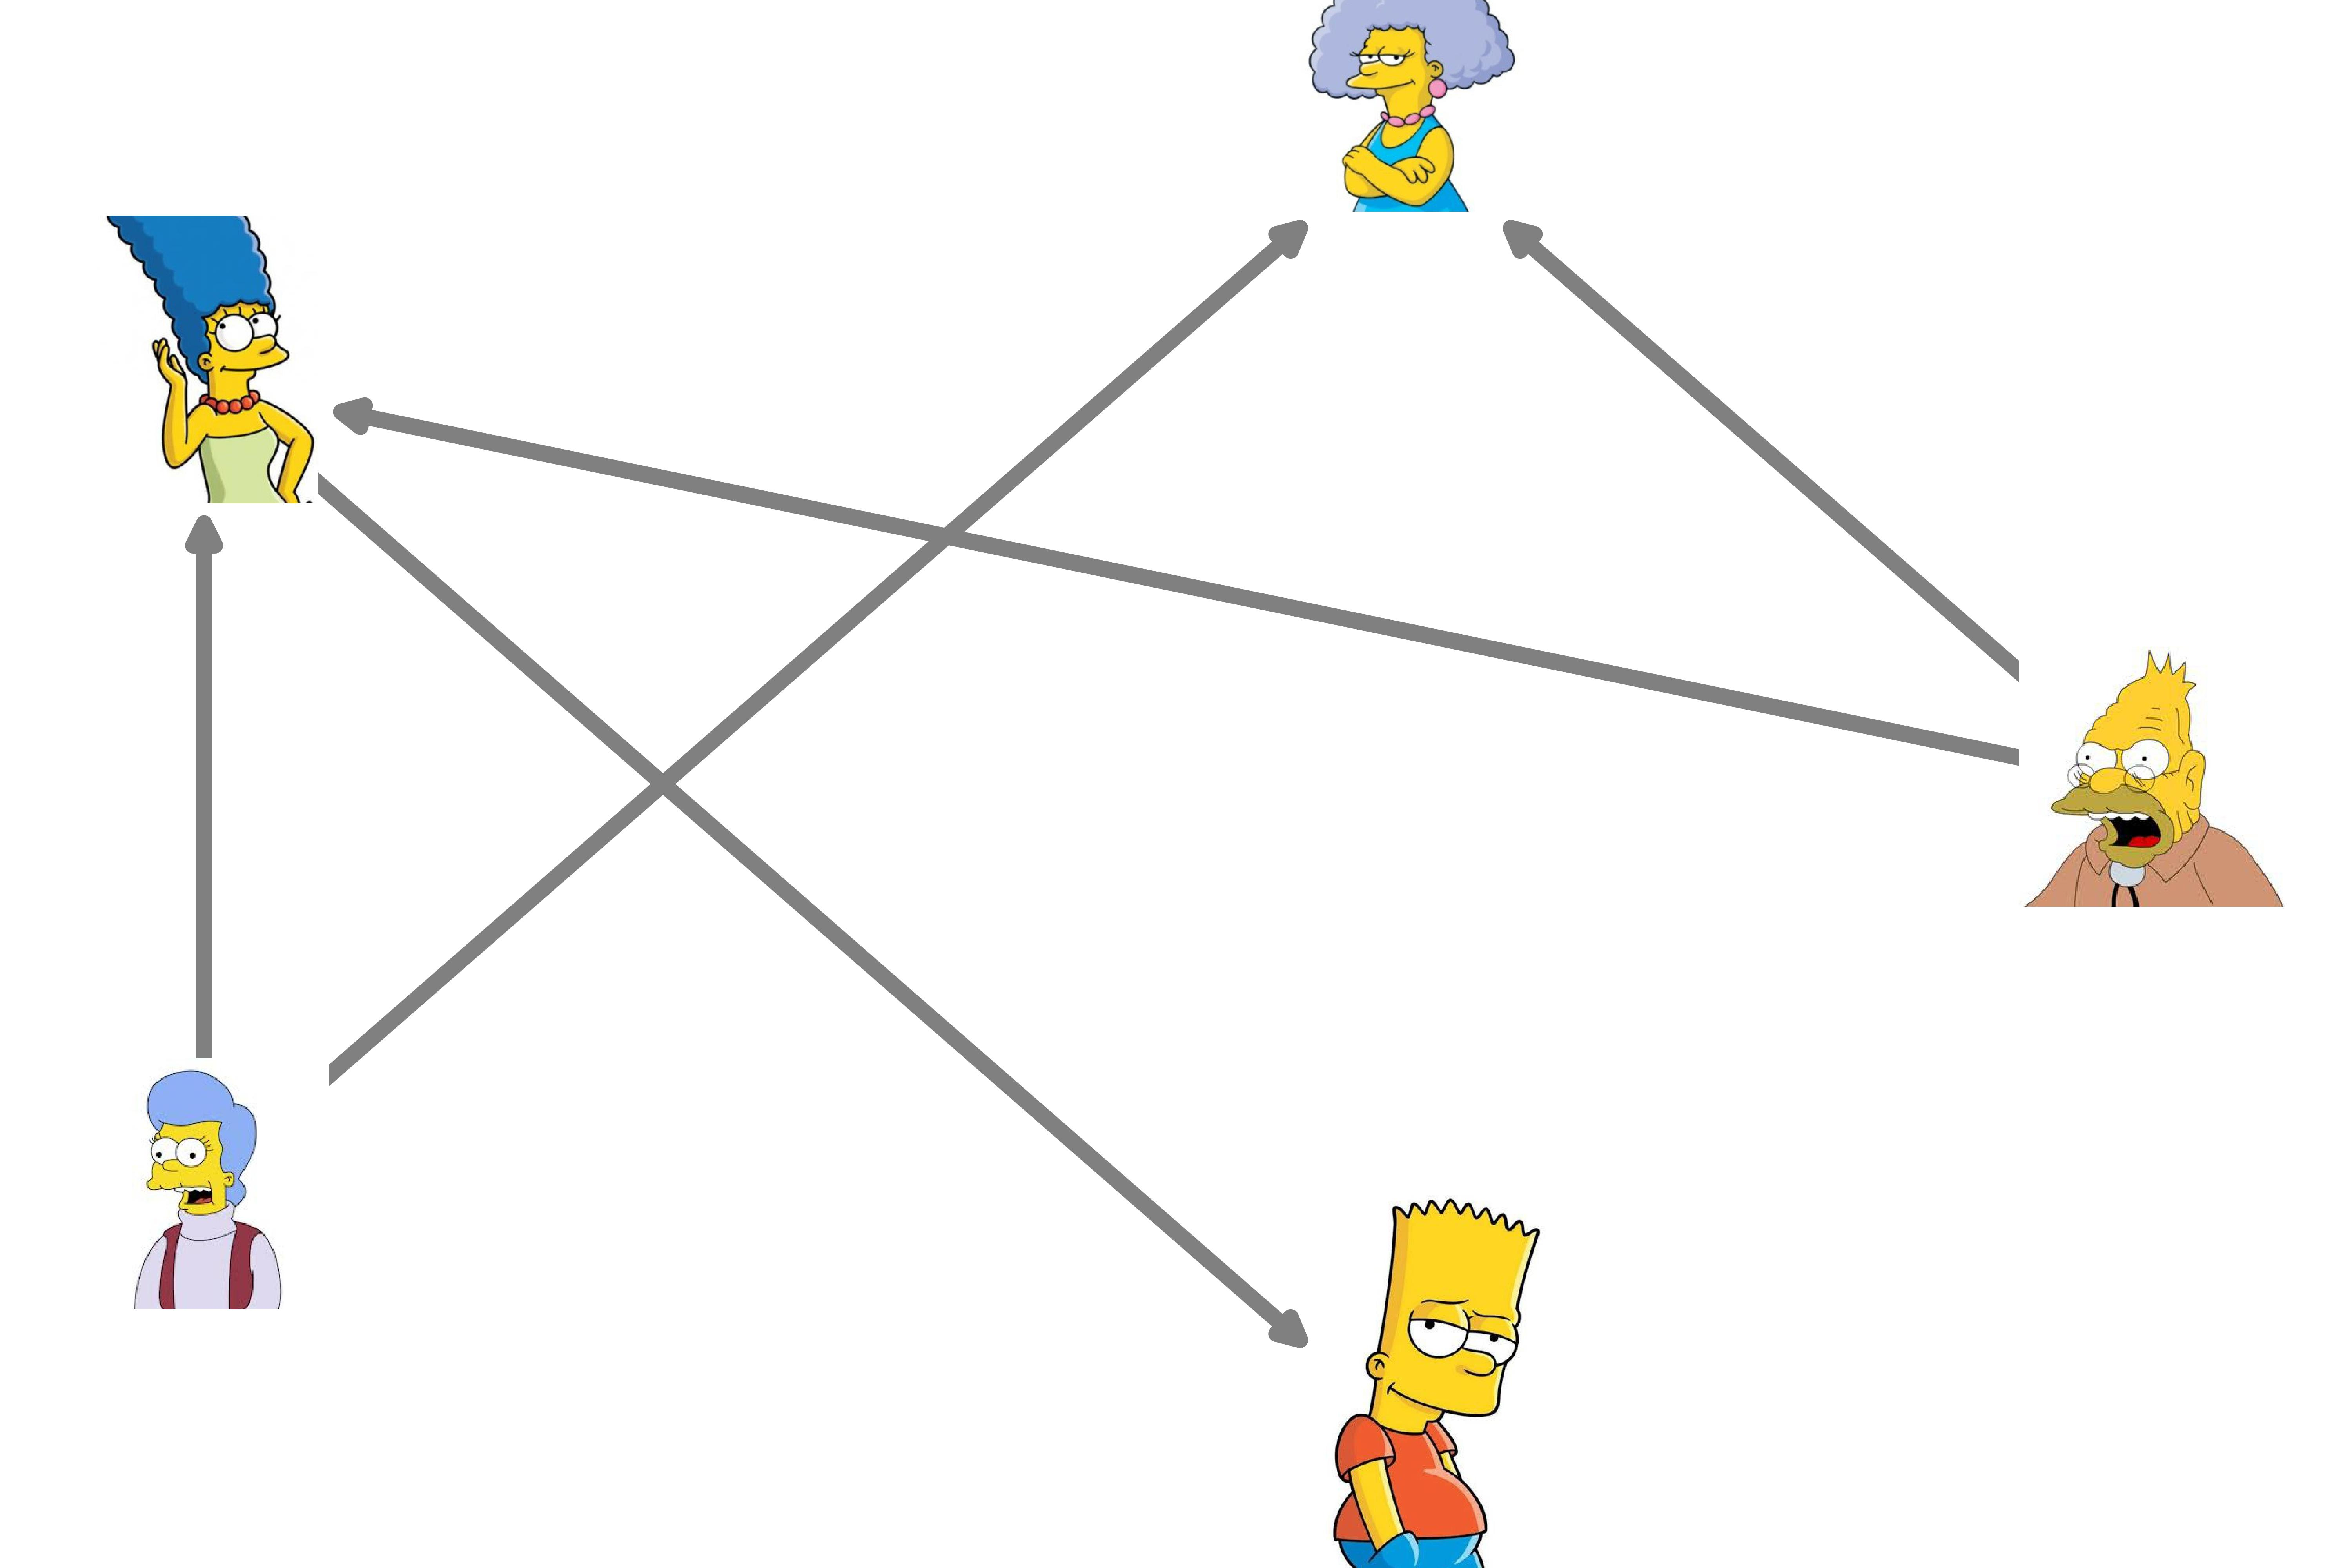
\includegraphics[width=80mm]{./grafo41}}
\subfigure[Rutas mas cortas de (a)]{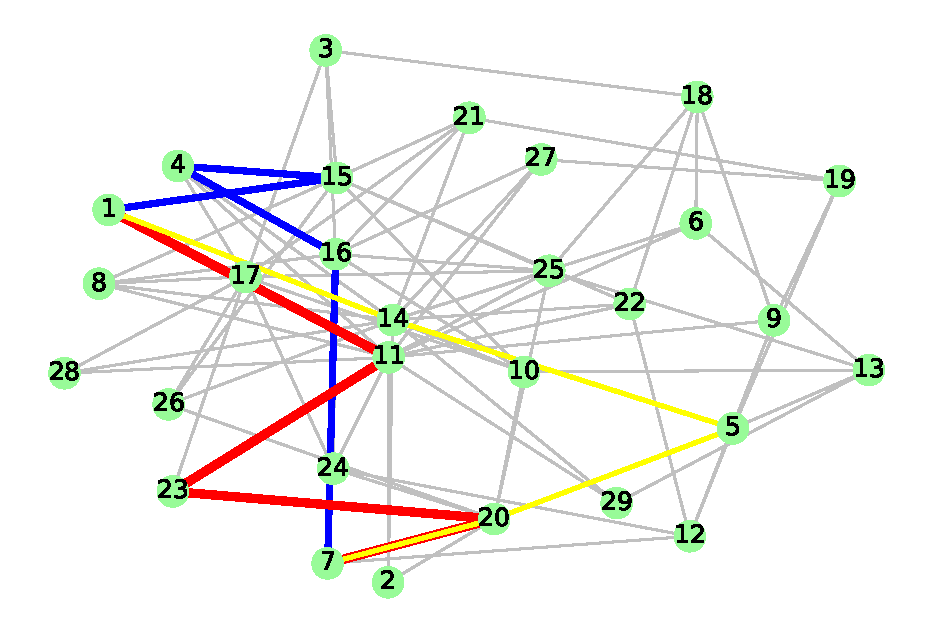
\includegraphics[width=80mm]{./grafo42}}
\caption{Ejemplo de rutas mas cortas} \label{figure7}
\end{figure}

Ahora se calcula para el algoritmo, el promedio y desviación estándar de la ejecución del conjunto de réplicas y se grafica un histograma.

\begin{figure}[H]
\centering
\subfigure[Histograma]{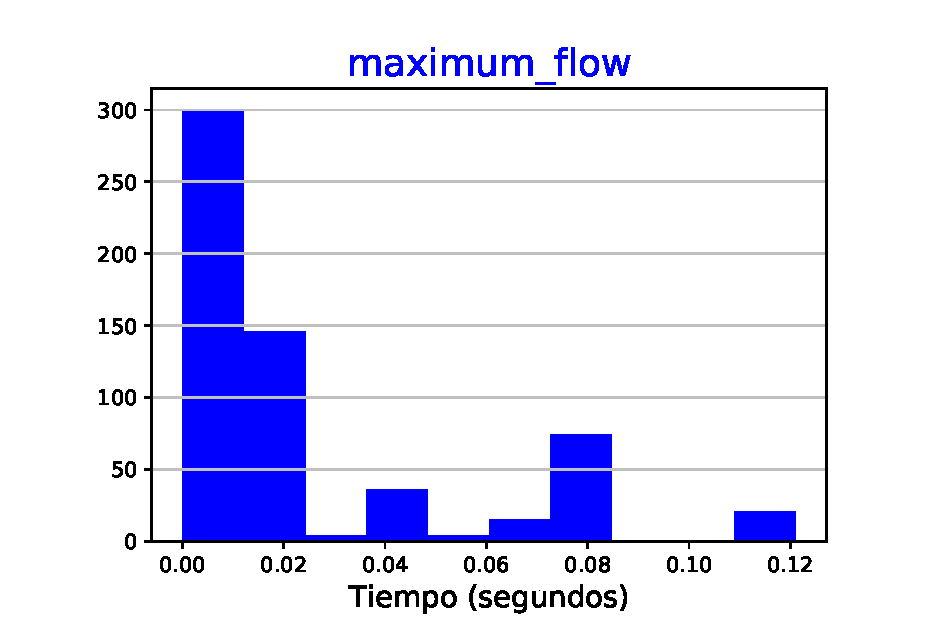
\includegraphics[width=70mm]{./histograma4}}
\subfigure[Diagrama de caja y bigotes]{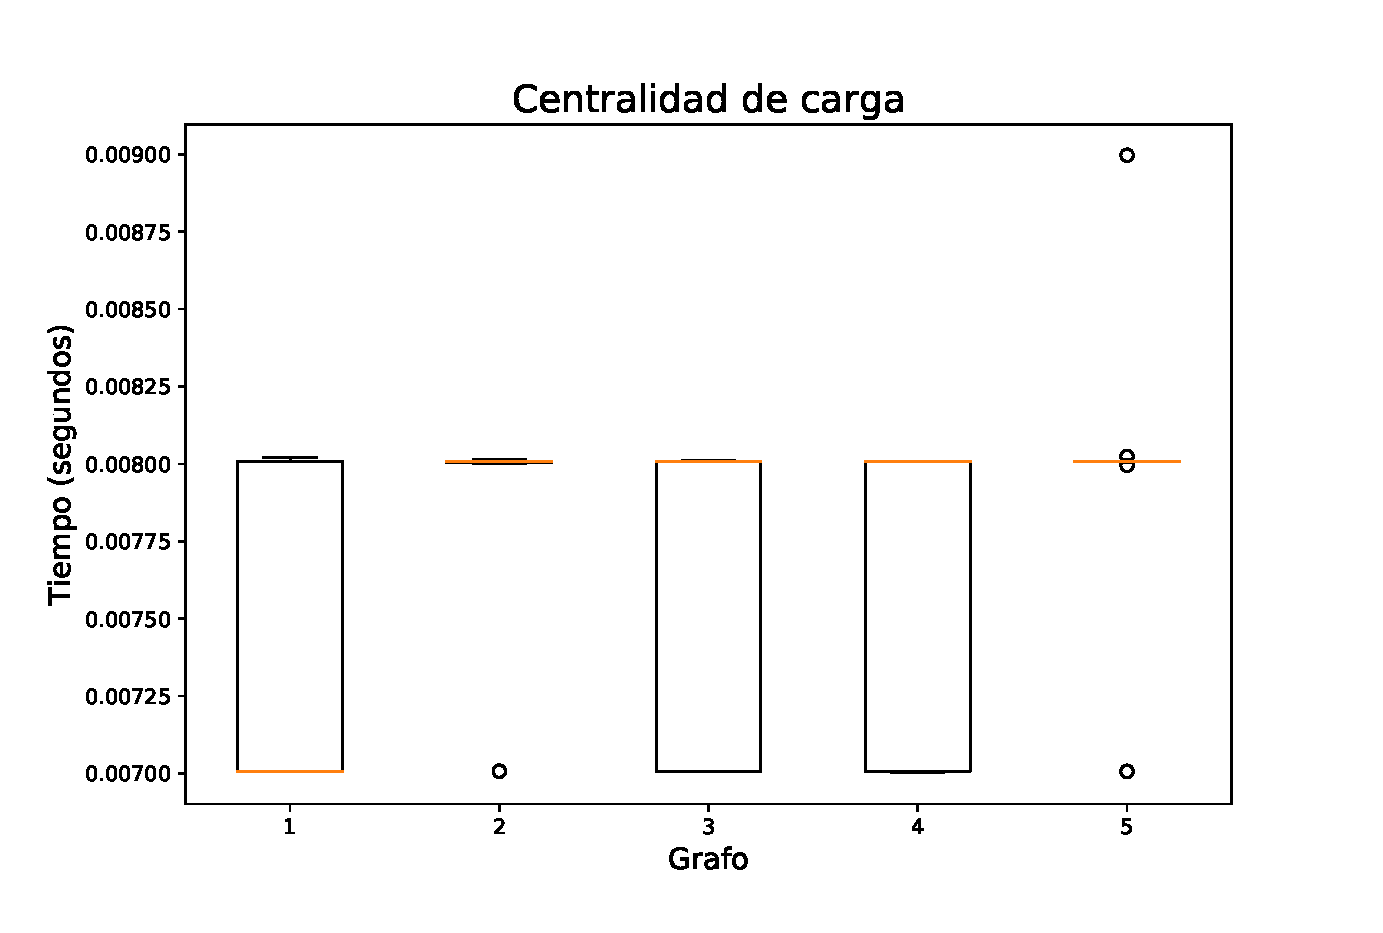
\includegraphics[width=90mm]{./boxplot4}}
\caption{Histograma y diagrama de caja y bigotes} \label{figure8}
\end{figure}

En la figura [\ref{figure8}.a] se muestra el histograma de los tiempos promedio del algoritmo y se calcula el promedio $(\mu)$ y la desviación estándar $(\sigma)$ para graficar la línea punteada que corresponde a la distribución normal $N\sim(\mu=5.70, \sigma=0.03)$ y se puede ver que la línea punteada no se ajusta al histograma por lo que se realiza la prueba estadística \textit{Shapiro-Wilk} para checar la normalidad de los datos.
\\
\\
\noindent\fbox{
\begin{minipage}{\textwidth}
\begin{algorithmic}
\State{\texttt{\color{blue}In:\color{black} \ stats.shapiro} (tiempos\_algoritmo\_4) \ \ \ \ \ \ \ \texttt{\color{blue}Out:\color{black} \ $(W=0.7345,p=  5.1768 \cdot {10}^{-6})$}}
\end{algorithmic}
\end{minipage}
}
\\
\\
La prueba muestra que el p-valor es menor a 0.05 (nivel de significancia), entonces la hipótesis nula es rechazada (se concluye que los datos no vienen de una distribución normal).
\\
\\
Por otro lado en la figura [\ref{figure8}.b] se muestran los diagramas de caja y bigotes para los tiempos individuales de los cinco grafos utilizados en el algoritmo, el número rojo representa la cantidad de nodos del grafo y se puede apreciar que conforme aumenta la cantidad de nodos en el grafo, los tiempos computacionales también crecen.






\subsection*{\centering{Coloración glotona}}

La figura [\ref{figure9}] muestra un ejemplo de un grafo y sus respectiva coloración propuesta por el algoritmo ejemplo.

\begin{lstlisting}[language=Python]
greedy1 = nx.coloring.greedy_color(G21, strategy='random_sequential')
\end{lstlisting}

\begin{figure}[H]
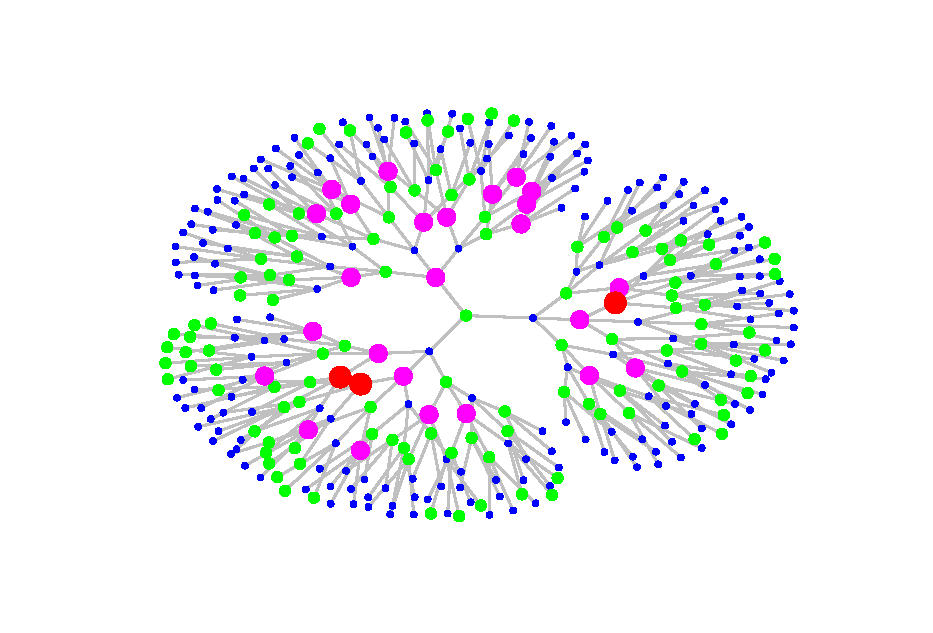
\includegraphics[width=150mm]{grafo52}
\caption{Ejemplo de coloración random} \label{figure9}
\end{figure}

Ahora se calcula para el algoritmo, el promedio y desviación estándar de la ejecución del conjunto de réplicas y se grafica un histograma.

\begin{figure}[H]
\centering
\subfigure[Histograma]{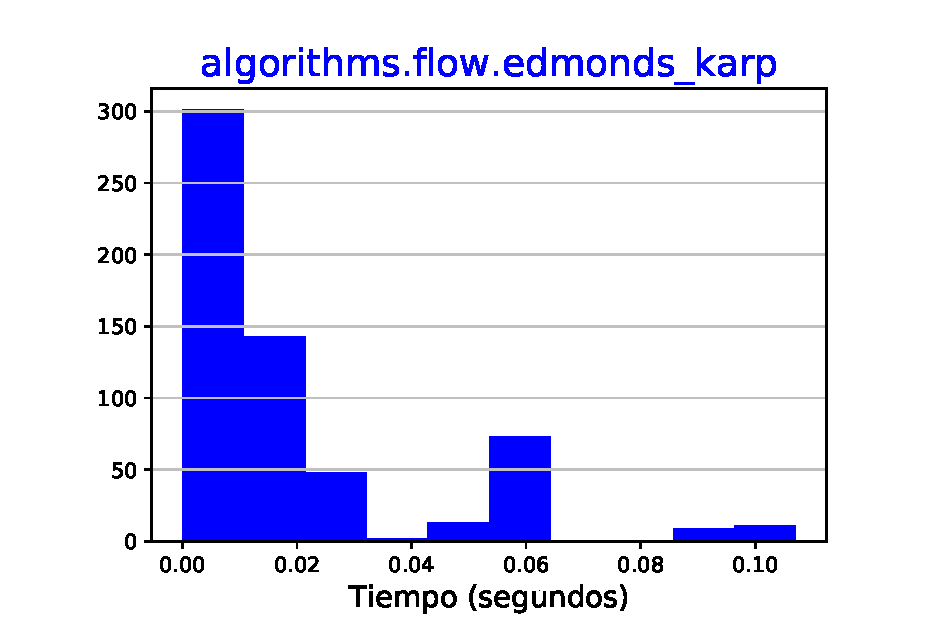
\includegraphics[width=70mm]{./histograma5}}
\subfigure[Diagrama de caja y bigotes]{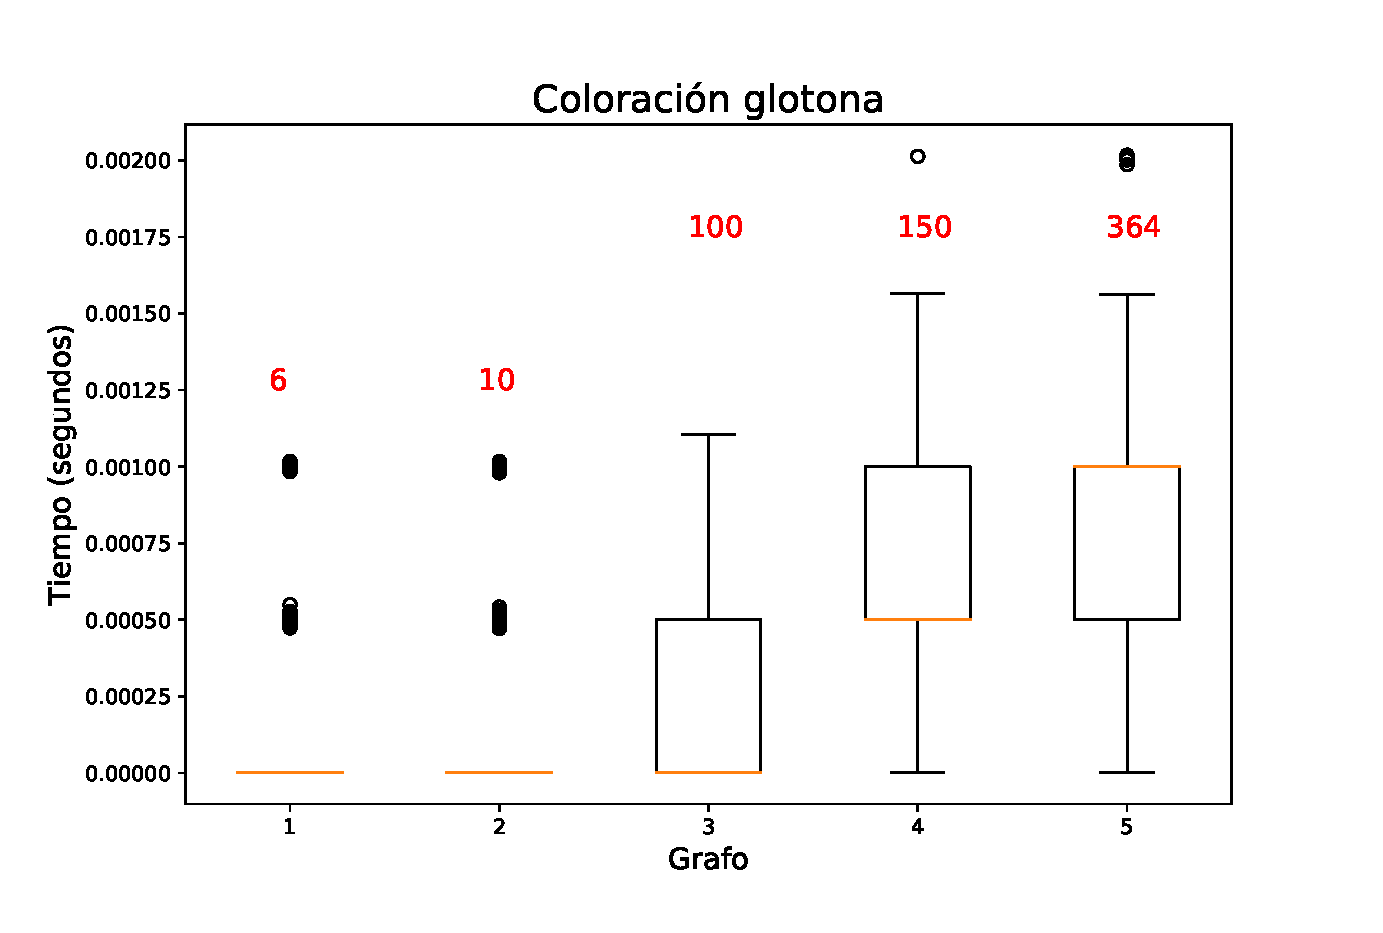
\includegraphics[width=90mm]{./boxplot5}}
\caption{Histograma y diagrama de caja y bigotes} \label{figure10}
\end{figure}

En la figura [\ref{figure10}.a] se muestra el histograma de los tiempos promedio del algoritmo y se calcula el promedio $(\mu)$ y la desviación estándar $(\sigma)$ para graficar la línea punteada que corresponde a la distribución normal $N\sim(\mu=5.18, \sigma=0.02)$ y se puede ver que la línea punteada no se ajusta al histograma por lo que se realiza la prueba estadística \textit{Shapiro-Wilk} para checar la normalidad de los datos.
\\
\\
\noindent\fbox{
\begin{minipage}{\textwidth}
\begin{algorithmic}
\State{\texttt{\color{blue}In:\color{black} \ stats.shapiro} (tiempos\_algoritmo\_5) \ \ \ \ \ \ \ \texttt{\color{blue}Out:\color{black} \ $(W=0.5863,p=  4.9988 \cdot {10}^{-8})$}}
\end{algorithmic}
\end{minipage}
}
\\
\\
La prueba muestra que el p-valor es menor a 0.05 (nivel de significancia), entonces la hipótesis nula es rechazada (se concluye que los datos no vienen de una distribución normal).
\\
\\
Por otro lado en la figura [\ref{figure10}.b] se muestran los diagramas de caja y bigotes para los tiempos individuales de los cinco grafos utilizados en el algoritmo, el número rojo representa la cantidad de nodos del grafo y se puede apreciar que conforme aumenta la cantidad de nodos en el grafo, los tiempos computacionales también crecen.
\\
\\
Además se incluyen dos gráficas de dispersión, en ambas el eje horizontal corresponde al tiempo promedio de ejecución de un algoritmo, contando con barras horizontales que representan la desviación estándar alrededor del punto que indica el promedio, mientras el eje vertical es el número de vértices del grafo en la primera gráfica, ver figura [\ref{figure11}] y el número de aristas en la segunda, ver figura [\ref{figure12}]; cada combinación de algoritmo-grafo se visualiza con un punto en la gráfica de dispersión (se distinguen entre algoritmos por colores y entre grafos por formas). 


\begin{figure}[H]
\centering
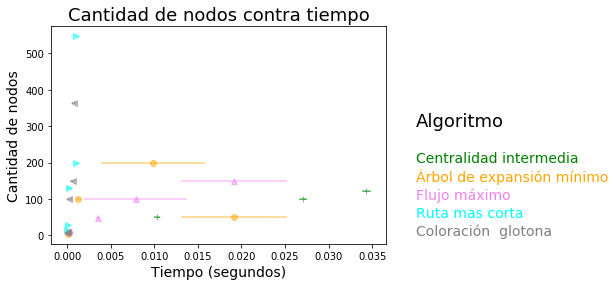
\includegraphics[width=130mm]{imagen1}
\caption{Cantidad de nodos contra tiempos} \label{figure11}
\end{figure}



\begin{figure}[H]
\centering
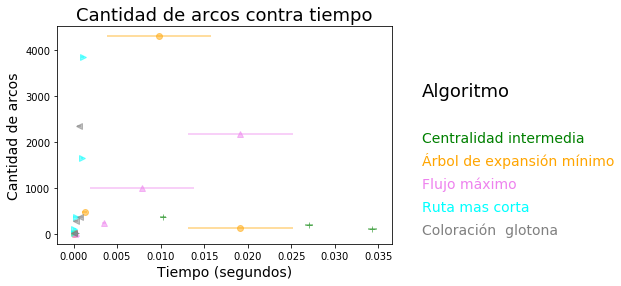
\includegraphics[width=130mm]{./imagen2}
\caption{Cantidad de arcos contra tiempos} \label{figure12}
\end{figure}






\bibliographystyle{unsrt}
\bibliography{biblio}
\nocite{*}

\end{document}